\chapter{\textit{Data Warehousing}}
\thispagestyle{chapterInit}

I sistemi di \textit{data warehousing} sono alla base di quasi tutti i \texttt{DSS} (\textit{Decision Support System}) e \texttt{BI} (\textit{Business Intelligence}) sono progettati per gestire grandi quantità di dati, per fornire un accesso rapido e per supportare le operazioni di analisi e di reporting.

\section{\textit{Data Warehouse} e metodologia \texttt{OLAP}}
    Prima della metodologia \texttt{OLAP} nasce la metodologia \texttt{OLTP} (\textit{On-Line Transaction Processing}) che è una tecnica di gestione dei dati per sistemi operazionali basata su 12 criteri.
    La metodologia \texttt{OLAP} (\textit{On-Line Analytical Processing}) è una tecnica di analisi dei dati iterativa.
    Negli anni i criteri per definire se un prodotto è \texttt{OLAP} o meno sono stati semplificati in 5 punti caratterizzati dall'acronimo \texttt{FASMI}:
    \begin{description}
        \item[\texttt{F}] \textit{Fast Analysis}: l'analisi deve essere veloce. (Tempo di risposta medio inferiore a 5 secondi)
        \item[\texttt{A}] \textit{Analytical} (Analitico): l'analisi deve essere analitica e deve:
            \subitem Dare la possibilità di eseguire nuovi calcoli a partire dai calcoli già eseguiti.
            \subitem Fornire risposte a richieste specifiche e non solo a domande predefinite.
            \subitem Fornire i dati in rappresentazioni molteplici.
        \item[\texttt{S}] \textit{Shared} (Condiviso): i dati devono essere utilizzabili da più utenti contemporaneamente che condividono la stessa base di dati di analisi.
        \item[\texttt{M}] \textit{Multidimensional} (Multidimensionale): i dati devono essere organizzati in modo multidimensionale.
        \item[\texttt{I}] \textit{Informational} (Informativo): il sistema deve contenere tutte le informazioni necessarie per l'analisi indipendentemente da dove e come sono memorizzate.
    \end{description}
\section{Architettura dei sistemi di \textit{data warehousing}}
    Un sistema di \textit{data warehousing} è costituito da basi di dati poste a livelli diversi, ognuno di questi ha una finalità, una struttura ed una tipologia di dati contenuti. Questi livelli sono:
    \begin{description}
        \item[Sorgenti] Sono le basi di dati operative (o esterne) da cui si estraggono i dati.
        \item[\textit{Staging Area}] È una area intermedia in cui i dati estratti dalle sorgenti vengono trasformati e caricati in una forma adatta per l'immagazzinamento presso la \textit{Data Warehouse}.
        \item[\textit{Data Warehouse}] È il livello in cui i dati vengono immagazzinati in modo da poter essere utilizzati per l'analisi.
        \item[\textit{Data Mart}] È un sottoinsieme del \textit{Data Warehouse} che contiene dati specifici per un determinato settore o per un determinato gruppo di utenti.
    \end{description}
    Elementi propri di un sistema sono oltre alle varie basi di dati:
    \begin{itemize}
        \item Procedure  che permettono di estrarre, trasformare e caricare i dati.
        \item Strumenti di analisi
    \end{itemize}
    \begin{figure}[H]
        \centering
        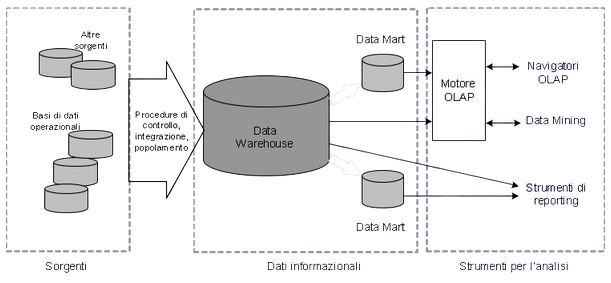
\includegraphics[width=0.7\textwidth]{08/livelliDW.png}
        \caption{Livelli di un sistema di \textit{data warehousing}}
    \end{figure}

\section{Modelli concettuali per il \textit{data warehouse}}
    I sistemi informazionali vista la quantità di informazioni contenute all'interno necessitano di modelli dati a descrivere la composizione del sistema e della sua base di dati. Viene dunque definito uno schema dei fatti, i \texttt{DFM} (\textit{Dimensional Fact Model}).
    \subsection{\textit{Dimensional Fact Model} - \texttt{DFM}}
        Il modello \texttt{DFM} viene usato per descrivere un fatto, tutte le sue misure e le dimensioni usabili per l'analisi (quelle sulle quali il fatto è aggregabile). Un \texttt{DFM} è composto da:
        \begin{itemize}
            \item Un fatto rappresentato tramite un rettangolo
            \item Le misure contenute nel fatto (sia quelle proprie che quelle derivate)
            \item Le dimensioni base collegate al fatto (le coordinate del fatto) rappresentate da cerchi
            \item Gli attributi descrittivi collegati o al fatto o alla dimensione.
            \item Le gerarchie tra le dimensioni sono rappresentate come un albero con la radice in alto.
                \subitem Se una gerarchia è condivisa tra più dimensioni si rappresenta con un cerchio pieno con $n$ collegamenti al fatto e alle dimensioni
            \item É possibile inoltre rappresentare le relazioni di aggregabilità tra misure e dimensioni. Queste relazioni sono rappresentate con una linea tratteggiata (se non è possibile aggregare) o continua (se è possibile aggregare).
        \end{itemize}
        \begin{figure}[H]
            \centering
            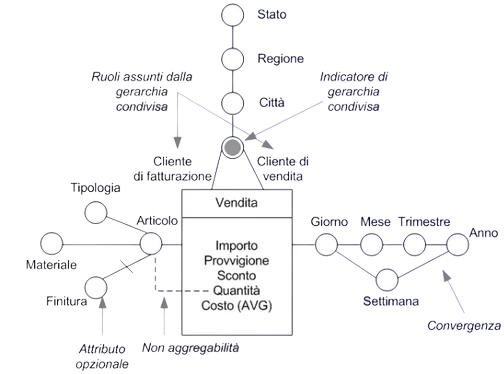
\includegraphics[width=0.5\textwidth]{08/DFM.png}
            \caption{Esempio di \texttt{DFM} con tutte le caratteristiche descritte}
        \end{figure}
        C'è da aggiungere che il presente modello è riconducibile ad un modello \texttt{E-R} (\textit{Entity-Relationship}) in cui le dimensioni sono le entità sono le entità e le gerarchie sono le relazioni tra le entità ed il fatto è l'entità principale.
\section{Modelli logici per il \textit{data warehouse}}
    Mentre la modellazione concettuale riguarda come i fatti e le dimensioni sono collegati tra loro, la modellazione logica riguarda come i fatti e le dimensioni sono effettivamente memorizzati nel \textit{Data Warehouse}. I modelli logici si differenziano sulla base della scelta del \texttt{DBMS} e della struttura di memorizzazione dei dati. Oltre a definire come i dati sono memorizzati, i modelli logici definiscono anche come i dati sono interrogati e analizzati.
    \subsection{\texttt{ROLAP}}
        Il modello \texttt{ROLAP} (\textit{Relational OLAP}) è un modello logico che prevede l'utilizzo di un \texttt{DBMS} relazionale e la memorizzazione viene eseguita tramite tabelle. Questo modello inoltre prevede che le interrogazioni avvengano tramite \textit{query} \texttt{SQL} con l'uso di viste e/o funzioni di aggregazione.
        \paragraph{Vantaggi} Ridotto uso di spazi di memorizzazione e la maggiore conoscenza degli strumenti relazionali portano ad una maggiore facilità di gestione.
        \paragraph{Svantaggi} Le prestazioni delle interrogazioni possono essere peggiori rispetto ad altri modelli e la complessità delle interrogazioni può aumentare se lavoriamo con diverse aggregazioni ed analisi.
    \subsection{\texttt{MOLAP}}
        Il modello \texttt{MOLAP} (\textit{Multidimensional OLAP}) è un modello logico che prevede l'utilizzo di strutture dati intrinsecamente multidimensionali. Questo modello prevede che i dati siano memorizzati in strutture multidimensionali (quali vettori, matrici, \dots) i sistemi allocano spazio per tutte le possibili combinazioni di dimensioni e misure.
        \paragraph{Vantaggi} Le prestazioni delle interrogazioni sono migliori rispetto ad altri modelli in quanto il fatto ricercato viene trovato in un'unica posizione e non è necessario ``simulare'' le dimensioni. Inoltre le operazioni di aggregazione sono più veloci in quanto si considera solo il livello di aggregazione richiesto.
        \paragraph{Svantaggi} L'uso di spazio di memorizzazione è maggiore rispetto ad altri modelli, solitamente solo il $20\%$ dello spazio allocato viene utilizzato. Inoltre non esiste uno standard, tutte le implementazioni sono proprietarie e non inter compatibili.
    \subsection{\texttt{HOLAP}} 
        Il modello \texttt{HOLAP} (\textit{Hybrid OLAP}) è un modello logico che prevede l'utilizzo di un \texttt{DBMS} relazionale e di strutture multidimensionali. Questo modello prevede che i dati siano memorizzati in strutture multidimensionali (per le aggregazioni di livello più alto) e in tabelle relazionali (per le aggregazioni di livello più basso). Le interrogazioni possono essere eseguite sia tramite \textit{query} \texttt{SQL} che tramite \textit{query} multidimensionali.
        \paragraph{Vantaggi} Questo modello permette di sfruttare i vantaggi di entrambi i modelli, inoltre permette di utilizzare le strutture multidimensionali per le aggregazioni di livello più alto e le tabelle relazionali per le aggregazioni di livello più basso. Infatti le \textit{data mart} possono essere memorizzati in modo multidimensionale mentre il \textit{data warehouse} può essere memorizzato in modo relazionale.
        \paragraph{Svantaggi} La complessità di gestione è maggiore rispetto ad altri modelli e le prestazioni delle interrogazioni possono essere peggiori rispetto ad altri modelli.
    \subsection{Schemi multidimensionali su basi di dati relazionali}
        Visto che la maggior parte delle \textit{data warehouse} vengono memorizzati in basi di dati relazionali, vediamo come è possibile implementare uno schema multidimensionale su una base di dati relazionale.
        \subsubsection{Schema a stella}
            Lo schema a stella è un modello multidimensionale in cui il fatto, le sue misure semplici e elementi ``chiave'' riguardanti le dimensioni sono memorizzati in una tabella centrale (il fatto), le dimensioni vere e proprie sono memorizzate in tabelle separate collegate al fatto tramite una chiave esterna. Questo modello è molto semplice e facile da implementare, inoltre è molto efficiente per le interrogazioni.
            \begin{figure}[H]
                \centering
                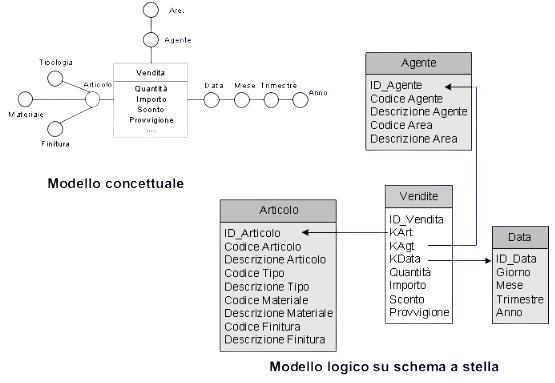
\includegraphics[width=0.5\textwidth]{08/stella.png}
                \caption{Schema a stella}
            \end{figure}
        \subsubsection{Schema a fiocco di neve} 
            Lo schema a fiocco di neve è un'estensione dello schema a stella in cui le tabelle delle dimensioni sono normalizzate. Questo modello permette di risparmiare spazio di memorizzazione in quanto le tabelle delle dimensioni sono più piccole, inoltre permette di ridurre la ridondanza dei dati. Tuttavia le interrogazioni possono essere più complesse e le prestazioni possono essere peggiori rispetto allo schema a stella.
            \begin{figure}[H]
                \centering
                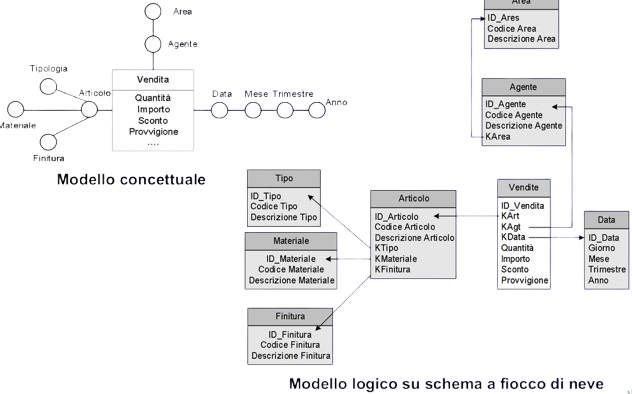
\includegraphics[width=0.5\textwidth]{08/fioccoDiNeve.png}
                \caption{Schema a fiocco di neve}
            \end{figure}
        \subsubsection{Costellazione di fatti}
            Lo schema a costellazione di fatti è un'estensione dello schema a stella in cui sono presenti più fatti collegati tra loro. Questo modello permette di analizzare più fatti contemporaneamente e di effettuare analisi più complesse. Tuttavia le interrogazioni possono essere più complesse e le prestazioni possono essere peggiori rispetto allo schema a stella.
            \begin{figure}[H]
                \centering
                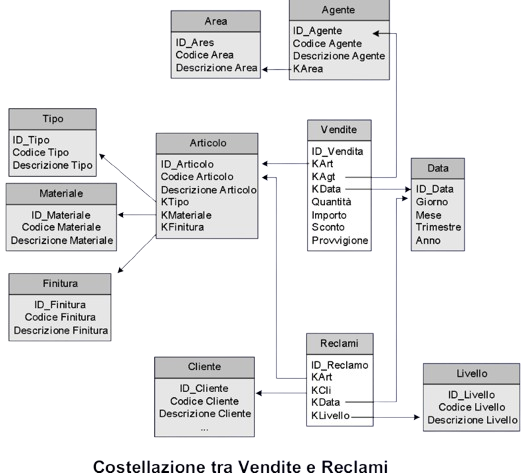
\includegraphics[width=0.5\textwidth]{08/costellazione.png}
                \caption{Schema a costellazione di fatti}
            \end{figure}
\section{Ciclo di vita di \texttt{DWH} e Popolazione del \texttt{DWH}}
    Andiamo ora a vedere come viene costruito un \texttt{DWH} e come vengono popolati i vari livelli.
    \subsection{Ciclo di vita di un \texttt{DWH}}
        La costruzione di una \texttt{DWH} è un processo iterativo che prevede diverse fasi:
        \begin{enumerate}
            \item Costruzione del primo ipercubo multidimensionale sul fatto più importante.
            \item Integrazione progressiva degli altri fatti
            \item Rilascio di \textit{data mart} per i vari settori aziendali
        \end{enumerate}
        Il vantaggio principale di questo approccio è che i primi risultati sono visibili in tempi brevi, gli investimenti sulla \texttt{DWH} sono diluiti nel tempo ed si può tarare il modello sulla base delle esigenze degli utenti.
    \subsection{Popolazione della \texttt{DWH}}
        La popolazione della \texttt{DWH} prevede diverse fasi:
        \begin{enumerate}
            \item Estrazione dei dati dalle sorgenti - i dati vengono estratti dalle sorgenti e trasferiti nella \texttt{DWH}
            \item Integrazione e trasformazione dei dati - associazione dei dati estratti con i dati già presenti nella \texttt{DWH}
            \item Pulizia dei dati - aumento della qualità
            \item Caricamento dei dati nella \texttt{DWH} - i dati vengono caricati nella \texttt{DWH}
        \end{enumerate}
        % TODO: Ci sarebbe da espandere un po' di più questa sezione ma non ho trovato tempo per farlo prima dell'esame ;)
\section{L'analisi \texttt{OLAP} e principali operatori \texttt{OLAP}}
    L'analisi \texttt{OLAP} è un'analisi iterativa che si basa sul paradigma dell'``esplorazione guidata delle ipotesi''. In sostanza una analisi \texttt{OLAP} prevede che in una stessa sessione di analisi ciascun passo è conseguenza dei risultati ottenuti al passo precedente, inoltre tutte le interrogazioni operano per differenza rispetto alla sessione precedente, ovvero il risultato di una interrogazione è la differenza tra il risultato dell'interrogazione corrente e il risultato dell'interrogazione precedente. I risultati finali sono presentati sotto forma di tabelle, grafici o mappe.
    \paragraph{Operatori \texttt{OLAP}}
    Gli operatori \texttt{OLAP} sono operatori che permettono di effettuare analisi sui dati. Gli operatori principali sono:
    \begin{description}
        \item[\textit{Drill Down}] Consente di passare da un livello di aggregazione ad un livello di dettaglio inferiore.
        \item[\textit{Roll Up}] Consente di passare da un livello di dettaglio ad un livello di aggregazione superiore.
        \item[\textit{Slice}] Consente di selezionare un sottoinsieme di dati su una dimensione.
        \item[\textit{Dice}] Consente di selezionare un sottoinsieme di dati su più dimensioni.
        \item[\textit{Pivot}] Consente di scambiare le righe con le colonne di una tabella oppure ruotare una rappresentazione grafica su un asse.
    \end{description}
    \subsubsection{\textit{Drill Down}}
        L'operatore \textit{Drill Down} consente di passare da un livello di aggregazione ad un livello di dettaglio inferiore. Questo operatore permette di visualizzare i dati in modo più dettagliato. Si può aggiungere una dimensione oppure si scende lungo una gerarchia. Graficamente andiamo a ``separare'' i dati in più sottoinsiemi, esempio possiamo passare da una tabella che mostra per la dimensione zona Nord Centro Sud il totale delle vendite per il 2020 ad una tabella che mostra per la dimensione delle regioni il totale delle vendite per il 2020. Siamo andati a ``separare'' i dati per regione e non più per zona.
    \subsubsection{\textit{Roll Up}}
        L'operatore \textit{Roll Up} è l'inverso dell'operatore \textit{Drill Down}, consente di passare da un livello di dettaglio ad un livello di aggregazione superiore. Questo operatore permette di visualizzare i dati in modo più aggregato. Si può rimuovere una dimensione oppure si sale lungo una gerarchia. Graficamente andiamo a ``unire'' i dati in un unico insieme, esempio possiamo passare da una tabella che mostra per la dimensione delle regioni il totale delle vendite per il 2020 ad una tabella che mostra per la dimensione zona Nord Centro Sud il totale delle vendite per il 2020. Siamo andati a ``unire'' i dati per zona e non più per regione.
    \subsubsection{\textit{Slice}}
        L'operatore \textit{Slice} consiste nel selezionare un sottoinsieme di dati su una dimensione. Questo significa che una volta determinato il valore che vogliamo selezionare, andiamo a ``tagliare'' i dati in modo che vengano visualizzati solo i dati che rispettano il valore selezionato. Tutte le altre dimensioni rimangono invariate.
    \subsubsection{\textit{Dice}}
        L'operatore \textit{Dice} è di base una combinazione di più operatori \textit{Slice}. Consente di selezionare un sottoinsieme di dati su più dimensioni. Questo significa che una volta determinati i valori che vogliamo selezionare, andiamo a ``tagliare'' i dati in un cubo in modo che vengano visualizzati solo i dati che per ogni dimensione rispettano il valore selezionato. Tutte le altre dimensioni rimangono invariate.
    \subsubsection{\textit{Pivot}}
        L'operatore \textit{Pivot} inverte la relazione tra le dimensioni andando a ruotare il cubo dell'analisi su un asse. Questo operatore consente di visualizzare i dati in modo differente, ad esempio possiamo passare da una tabella che mostra per la dimensione zona Nord Centro Sud il totale delle vendite per il 2020 ad una tabella che mostra per la dimensione delle regioni il totale delle vendite per il 2020. Siamo andati a ``ruotare'' i dati su un asse.
    